\section{Cardinalit\`a}
Il concetto di cardinalit\`a \`e, forse, il modo pi\`u semplice di contare gli elementi di un insieme: diciamo che due insiemi hanno un ugual numero di elementi se esiste
una corrispondenza biunivoca fra di essi.

\begin{definition}[Equipotenza/Cardinalit\`a]
	Dati due insiemi $A$ e $B$:
\begin{align*}
{\drkblu |A| = |B|} \;\;\Mydef\;\;& \exists {f \in {}^A B} \;\; \text{``$f$ \`e bigettiva $A \to B$''}\\[-\jot]
\text{\drkgrn ``$A$ ha la stessa \vocab{cardinalit\`a} di $B$''}\phantom{\;\;\Mydef\;\;}&\\[-\jot]
\text{\drkgrn ``$A$ e $B$ sono \vocab{equipotenti}''}\phantom{\;\;\Mydef\;\;}&\\[-\jot]
\\[-\jot]
{\drkblu |A| \leq |B|} \;\;\Mydef\;\;& \exists {B' \subseteq B} \; |A| = |B'|\\[-\jot]
\text{\drkgrn ossia:}\;&\exists {f \in {}^A B} \;\;\text{``$f$ \`e iniettiva''}
\end{align*}
\end{definition}

\begin{note}
\ 
\vskip-3\baselineskip
\ 
	\begin{itemize}
		\item La scrittura $|A| = |B|$ suggerisce che esistano insiemi -- o, comunuqe, oggetti di qualche genere -- denotati $|A|$ e~$|B|$ di cui si predica l'uguaglianza.
		Effettivamente costruiamo questi oggetti, ma, per ora, la
scrittura $|A| = |B|$ \`e inscindibile, come $\mouse(A,B)$.
		\item Ci sentiremo liberi di scrivere
$|A|\ge|B|$ e $|A|\neq|B|$ per indicare $|B|\le|A|$ e~$\neg\,|A|=|B|$
rispettivamente.
		\item Se $A\subseteq B$ vale anche $|A|\le|B|$. Tuttavia,
se $A \subsetneq B$ non \`e detto che valga la
disuguaglianza stretta~$|A|<|B|$, come mostra l'esempio di $A = \{x \in \omega | x > 0\}$ e $B = \omega$.
	\end{itemize}
\end{note}

\begin{remark}
	La relazione $|\cdot| = |\cdot|$ soddisfa le propriet\`a formali
di una relazione di equivalenza:\\
{\drkblu Riflessivit\`a:} $|A| = |A|$.\\
{\drkblu Simmetria:} $|A| = |B| \rightarrow |B| = |A|$.\\
{\drkblu Transitivit\`a:} $|A| = |B| \land |B| = |C| \rightarrow |A| = |C|$.
\end{remark}

\begin{exercise}
	Dimostrare l'osservazione.
\end{exercise}

\begin{remark}
	La relazione $|\cdot| \leq |\cdot|$ soddisfa:\\
{\drkblu Riflessivit\`a:} $|A| \leq |A|$.\\
{\drkblu Transitivit\`a:} $|A| \leq |B| \land |B| \leq |C| \rightarrow |A|
\leq |C|$.\\
\`E inoltre {\drkblu compatibile con la relazione~$|\cdot| = |\cdot|$:}
$|A|=|B|\rightarrow |A|\le|B|$.
\end{remark}

\begin{exercise}
	Dimostrare l'osservazione.
\end{exercise}

Per stabilire che le cardinalit\`a sono, formalmente, ordinate dalla
relazione $|\cdot| \leq |\cdot|$, ci manca l'antisimmetria, e questo \`e
l'enunciato del teorema di Cantor-Bernstein.

\subsection{Teorema di Cantor-Bernstein}
\ 

\begin{theorem}
	[Cantor-Bernstein]
	\label{CB}
\ 
\vskip-2\baselineskip
	\[ \forall {A,B} \;\; (|A| \leq |B| \land |B| \leq |A|)
\;\rightarrow\; |A| = |B|
		\]
	{\drkgrn Se c'\`e una funzione iniettiva $A \rightarrow B$ e una
funzione iniettiva $B \rightarrow A$, allora esiste una bigezione fra $A$
e $B$.}
\end{theorem}

\begin{proof}
	Siano $f\colon A \to B$ e $g\colon B \to A$ iniettive. Il nostro
obiettivo \`e costruire una nuova funzione $h \colon A \to B$ bigettiva.

{\def\maf{\;\;{\color{violet} \overset{f}{\mapsto}}\;\;}
\def\mag{\;\;{\color{blue!50!cyan} \overset{g}{\mapsto}}\;\;}
\drkgrn L'idea \`e che ogni elemento, poniamo, di $A$, \`e una tappa di un percorso:
\[\color{black} a \maf f(a) \mag g(f(a)) \maf f(g(f(a))) \mag \dots \]
	Siccome $f$ e $g$ sono iniettive, questo percorso ha altres\`i
un'unica estensione all'indietro:
	\[ \drkred \dots\mag f^{-1}(g^{-1}(a)) \maf g^{-1}(a) \mag
\color{black} a \maf f(a) \mag g(f(a)) \maf f(g(f(a)))
\mag \dots
		\]
	a patto che $a \in \Imm(g)$), $g^{-1}(a) \in \Imm(f)$, \etc. Quando, e se, non possiamo pi\`u applicare la funzione inversa, il percorso all'indietro si interrompe.
	Ci sono quindi solo tre tipi di percorsi possibili:
	\begin{figure}[H]
		\centering
		\includegraphics[width=\textwidth]{immagini/cantor-ber1a.png}
	\end{figure}
	\begin{figure}[H]
		\centering
		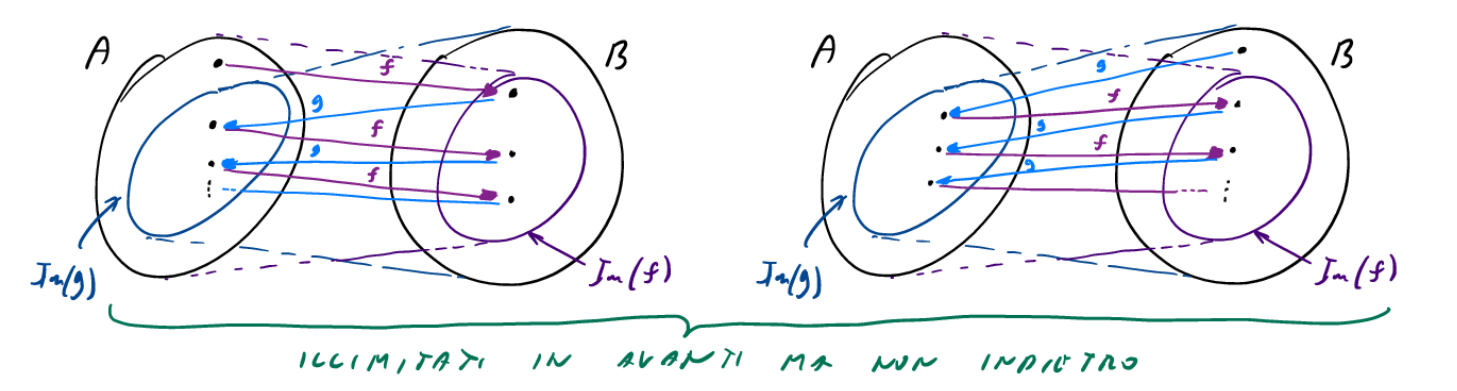
\includegraphics[width=\textwidth]{immagini/cantor-ber1b.png}
	\end{figure}
	Per gli elementi che si trovano su un percorso circolare, o su un
percorso illimitato avanti e indietro, $f$ fornisce una bigezione, come la
fornirebbe anche $g^{-1}$ -- la scelta \`e arbitraria a patto di 
	usare la medesima funzione per l'intero percorso.
	\begin{figure}[H]
		\centering
		\includegraphics[width=\textwidth]{immagini/cantor-ber2a.png}
	\end{figure}
\vskip-.7cm
	\begin{figure}[H]
		\centering
		\includegraphics[width=\textwidth]{immagini/cantor-ber2b.png}
	\end{figure}
	Per i percorsi illimitati solo in avanti, occorre invece vedere in quale insieme sta l'elemento iniziale del percorso: se questo \`e in $A$, la bigezione \`e data da $f$,
	altrimenti se sta in $B$ la bigezione \`e data da $g^{-1}$.
	\begin{figure}[H]
		\centering
		\includegraphics[width=\textwidth]{immagini/cantor-ber3.png}
	\end{figure}
	Per comodit\`a poniamo quindi $h(x) = f(x)$ in ogni caso, eccetto quando $x$ \`e lungo un percorso che parte da $B$, nel cui caso poniamo $h(x) = g^{-1}(x)$.}

	Formalmente, definiamo per \hyperref[ric1]{ricorsione} le seguenti
successioni di sottoinsiemi di $B$ e $A$ rispettivamente -- ossia,
tecnicamente, la funzione $\omega \to \ps(B) \times \ps(A) \colon i
\mapsto (B_i,A_i)$.
	\[ B_0 = B \setminus\Imm(f) \qquad A_i = g[B_i] \qquad B_{s(i)} = f[A_i]
		\]
	Definiamo quindi:
	\[ B_* = {\drkred \bigcup_{i \in \omega}B_i} \Mydef \bigcup\{B_i | i \in \omega\} \qquad A_* = \bigcup_{i \in \omega} A_i
		\]
	Gli elementi di $B_*$ e~$A_*$ sono i punti appartenenti a cammini
che partono da $B$, definiamo quindi $h\colon A \to B$ e $k\colon B \to A$ come segue:
	\[ h(x) = \begin{cases}
		g^{-1}(x) &\text{se $x \in A_*$}\\
		f(x) &\text{altrimenti}
	\end{cases}
	\qquad
	k(y) = \begin{cases}
		g(y) &\text{se $y \in B_*$}\\
		f^{-1}(y) &\text{altrimenti}
	\end{cases}
		\]
	Ci basta dimostrare che $h$ e $k$ sono ben definite, $k \circ h = \id_A$ e $h \circ k = \id_B$.

{\drkblu Buona definizione di $h$ e $k$.} Occorre verificare che stiamo applicando $g^{-1}$ e $f^{-1}$ a elementi della immagine di $g$ e $f$ rispettivamente.
		Nella definizione di $h$, se $x \in A_*$, allora $x \in A_i$, per qualche $i \in \omega$, quindi $x \in g[B_i] \subseteq \Imm(g)$. Nella definizione di $k$, se $y \not \in B_*$, in particolare,
		$y \not \in B_0$, per cui $y \in \Imm(f)$.

{\drkblu $k \circ h = \id_A$.} Se $x \in A_*$, allora $x \in A_i$, per qualche $i \in \omega$, quindi $x = g(y)$, con $y \in B_i$, per cui $k(h(x)) = k(g^{-1}(x)) = k(y) = g(y) = x$.
		Per il caso $x \not \in A_*$, osserviamo, intanto, che $x \not \in A_* \implies f(x) \not \in B_*$. Infatti, se $f(x) \in B_i$, con $i \in \omega$, allora $i \ne 0$, perch\'e $B_0 = B \setminus \Imm(f)$, quindi possiamo scrivere $i = s(j)$, 
		e $f(x) \in B_{s(j)} = f[A_j]$. Per l'iniettivit\`a di
$f$, abbiamo allora $x \in A_j \;\lightning\,$
		Di conseguenza, se $x \not \in A_*$, $k(h(x)) = k(f(x)) = f^{-1}(f(x)) = x$.

{\drkblu $h \circ k = \id_B$.} Se $y \in B_*$, allora $y \in B_i$, per qualche $i \in \omega$, quindi $g(y) \in A_i$. Di conseguenza $h(k(y)) = h(g(y)) = g^{-1}(g(y)) = y$. Altrimenti $y \not \in B_*$ e, se $f^{-1}(y)\in A_*$, avremmo una contraddizione,
		perch\'e $f^{-1}(y) \in A_i \rightarrow y = f(f^{-1}(y)) \in A_{s(i)}$. Quindi $h(k(y)) = h(f^{-1}(y)) = f(f^{-1}(y)) = y$.
\end{proof}

Visto che $|\cdot|\leq|\cdot|$ ha le propriet\`a formali di una relazione d'ordine fra le classi di equivalenza della relazione $|\cdot| = |\cdot|$, possiamo definire il corrispondente ordine stretto.

\begin{definition}
	Dati due insiemi $A$ e $B$ definiamo:
	\[ {\drkblu |A| < |B|} \;\;\Mydef\;\; |A| \leq |B| \land |A| \neq |B| \]
\end{definition}

% PIPPO

\subsection{Teorema di Cantor}

\ 

\begin{theorem}[Cantor]
	\label{cantor}
	Dato un insieme qualunque $A$, vale $|A| < |\ps(A)|$.
\end{theorem}

{\drkgrn La dimostrazione di questo enunciato \`e, ancora una volta, il
medesimo argomento del paradosso di Russell.}

\begin{proof}
	La disuguaglianza $|A| \leq |\ps(A)|$ \`e facile: basta considerare la funzione iniettiva
	$A \to \ps(A)$ che manda $x$ in~$\{x\}$

	Consideriamo, ora, una funzione arbitraria $f\colon A \rightarrow \ps(A)$.
	Ci basta dimostrare che $f$ non pu\`o essere surgettiva. Consideriamo:
	\[ B = \{x \in A | x \not \in f(x)\} \]
	Supponendo, per assurdo, che $f$ sia surgettiva, avremmo $B = f(a)$
per qualche $a \in A$. Quindi
	\[ a \in f(a) \;\;\iff\;\; a \in B \;\;\iff\;\; a \not \in f(a)
\quad \lightning
		\]
\end{proof}

\subsection{Operazioni fra cardinalit\`a}

\ 

\begin{definition}[Unione disgiunta]
	\[ {\drkblu A \sqcup B} \;\;\Mydef\;\; (A \times \{0\}) \cup (B \times
\{1\}) \]
\end{definition}

\begin{definition}[Somma, prodotto e potenza di cardinalit\`a]
	\[ {\drkblu |A| + |B|} \;\;\Mydef\;\; |A \sqcup B| \qquad {\drkblu |A|\cdot |B|
}\;\;\Mydef\;\; |A \times B| \qquad
		{\drkblu |A|^{|B|}} \;\;\Mydef\;\; |{}^{B}A|
		\]
\end{definition}

\begin{proposition}
	Le operazioni di somma, prodotto e potenza di cardinalit\`a sono ben definite, ossia dati $A,B,A',B'$, con $|A| = |A'|$ e $|B| = |B'|$, vale:
	\[ |A| + |B| \;\;=\;\; |A'| + |B'| \qquad |A|\cdot|B| \;\;=\;\;
|A'|\cdot|B'| \qquad |A|^{|B|} \;\;=\;\; |A'|^{|B'|}
		\]
\end{proposition}

\begin{proof}
	Date $f : A \rightarrow A'$ e $g : B \rightarrow B'$ bigettive, \`e immediato verificare che le seguenti sono bigezioni:
\begin{align*}
\drkred A \sqcup B &\drkred \to A' \sqcup B' &\drkred A \times B
&\drkred\to A' \times B' &\drkred {}^{B}A &\drkred\to
{}^{B'}A' \\
(a,0) &\mapsto (f(a),0) & (a,b) &\mapsto (f(a),g(b)) & h &\mapsto f \circ
h \circ g^{-1} \\
(b,1) &\mapsto (g(b),1)
\end{align*}
\vskip-\baselineskip
\end{proof}

\begin{notation}[Cardinalit\`a finite]
Riferendoci alle cardinalit\`a finite $|\emptyset|,|1|,|2|,\ldots$ se non c'\`e rischio di confusione, scriveremo semplicemente $0,1,2,\ldots$
\end{notation}

\begin{remark}
	$|\ps(A)| = 2^{|A|}$, per cui il \hyperref[cantor]{teorema di Cantor} pu\`o essere enunciato dicendo che, dato un qualunque $A$, vale $|A| < 2^{|A|}$.
\end{remark}

\begin{proof}
	La funzione che ad ogni $B \in \ps(A)$ associa la sua
\vocab{funzione indicatrice} $\chi_B\colon A \rightarrow 2$ definita da:
	\[ \chi_B(x) = \begin{cases}
		1 &\text{se $x \in B$}\\
		0 &\text{altrimenti}
	\end{cases}
		\]
	\`e una bigezione $\ps(A) \rightarrow {}^{A}2$.
\end{proof}

\begin{proposition}
	Le operazioni fra cardinalit\`a godono delle propriet\`a seguenti: denotando, per brevit\`a, con $\alpha,\beta,\gamma$ i simboli $|A|,|B|,|C|$
	\begin{align*}
\alpha + 0 &= \alpha 	 & \alpha + \beta &= \beta + \alpha
& \alpha + (\beta + \gamma) &= (\alpha + \beta) + \gamma \\
\alpha \cdot 0 &= 0 	 & \alpha \cdot \beta &= \beta \cdot \alpha 	&
\alpha \cdot (\beta \cdot \gamma) &= (\alpha \cdot \beta) \cdot \gamma \\
\alpha \cdot 1 &= \alpha & \mathrlap{\quad\;\;\alpha \cdot (\beta + \gamma) =
\alpha \cdot \beta + \alpha \cdot \gamma} \\
\alpha^0 &= 1 		& (\alpha^\beta)^\gamma &= \alpha^{\gamma \cdot
\beta} & (\alpha \cdot \beta)^\gamma &= \alpha^\gamma \cdot \beta^\gamma \\
\alpha^1 &= \alpha	& \alpha^{\beta + \gamma} &= \alpha^\beta \cdot
\alpha^\gamma \\
1^\alpha &= 1
	\end{align*}
\end{proposition}

\begin{proof}
	In ciascun caso, si tratta semplicemente di esibire una bigezione esplicita fra il membro di sinistra e il membro di destra. Come esempio, vediamo uno dei casi pi\`u complicati, il resto 
	\`e lasciato come {\drkred esercizio}.

	Dimostriamo che $(|A|^{|B|})^{|C|} = |A|^{|C|\cdot|B|}$. Dobbiamo esibire una bigezione fra l'insieme ${}^C({}^BA)$ delle funzioni che ad ogni elemento di $C$ associano una funzione $B \rightarrow A$, e l'insieme ${}^{C \times B}A$, delle funzioni 
	che ad ogni coppia di elementi in $C \times B$ associano un elemento di $A$. Associamo a $f \in {}^C({}^BA)$ la funzione $\widetilde{f} \in {}^{C \times B}A$ definita da:
	\[ \widetilde{f}(c,b) \;\;=\;\; f(c)(b) \]
	Dimostriamo che l'inversa di questa applicazione associa a $g \in {}^{C \times B}A$ la funzione $\overline{g} \in {}^{C}({}^B A)$ definita da:
	\begin{align*}
\overline{g}(c) \colon B &\to A \\
b &\mapsto g(c,b)
\end{align*}
	La verifica \`e facilissima, prese $f\in{}^{C}({}^B A)$ e $g \in {}^{C \times B}A$ si ha:
\begin{alignat*}{2}
	\forall {c\in C}\;\forall {b \in B} \quad
&\overline{\widetilde{f}}(c)(b) = \widetilde{f}(c,b) = (f(c))(b)
&&\;\;\implies\;\; \overline{\widetilde{f}}(c) = f(c)\\
	\forall {(c,b) \in C \times B} \quad
&\widetilde{\overline{g}}(c,d) = (\overline{g}(c))(b) = g(c,b)
&&\;\;\implies\;\; \widetilde{\overline{g}} = g
\end{alignat*}
\vskip-2\baselineskip
\end{proof}
